\subsection{Election November 5, 1916: *Wilson vs Hughes}
\begin{frame}[t]{Election November 7, 1916: *Woodrow Wilson}
\small
% Wilson
\begin{columns}[T, onlytextwidth]
\column{0.48\textwidth}
\vspace{-1em}
{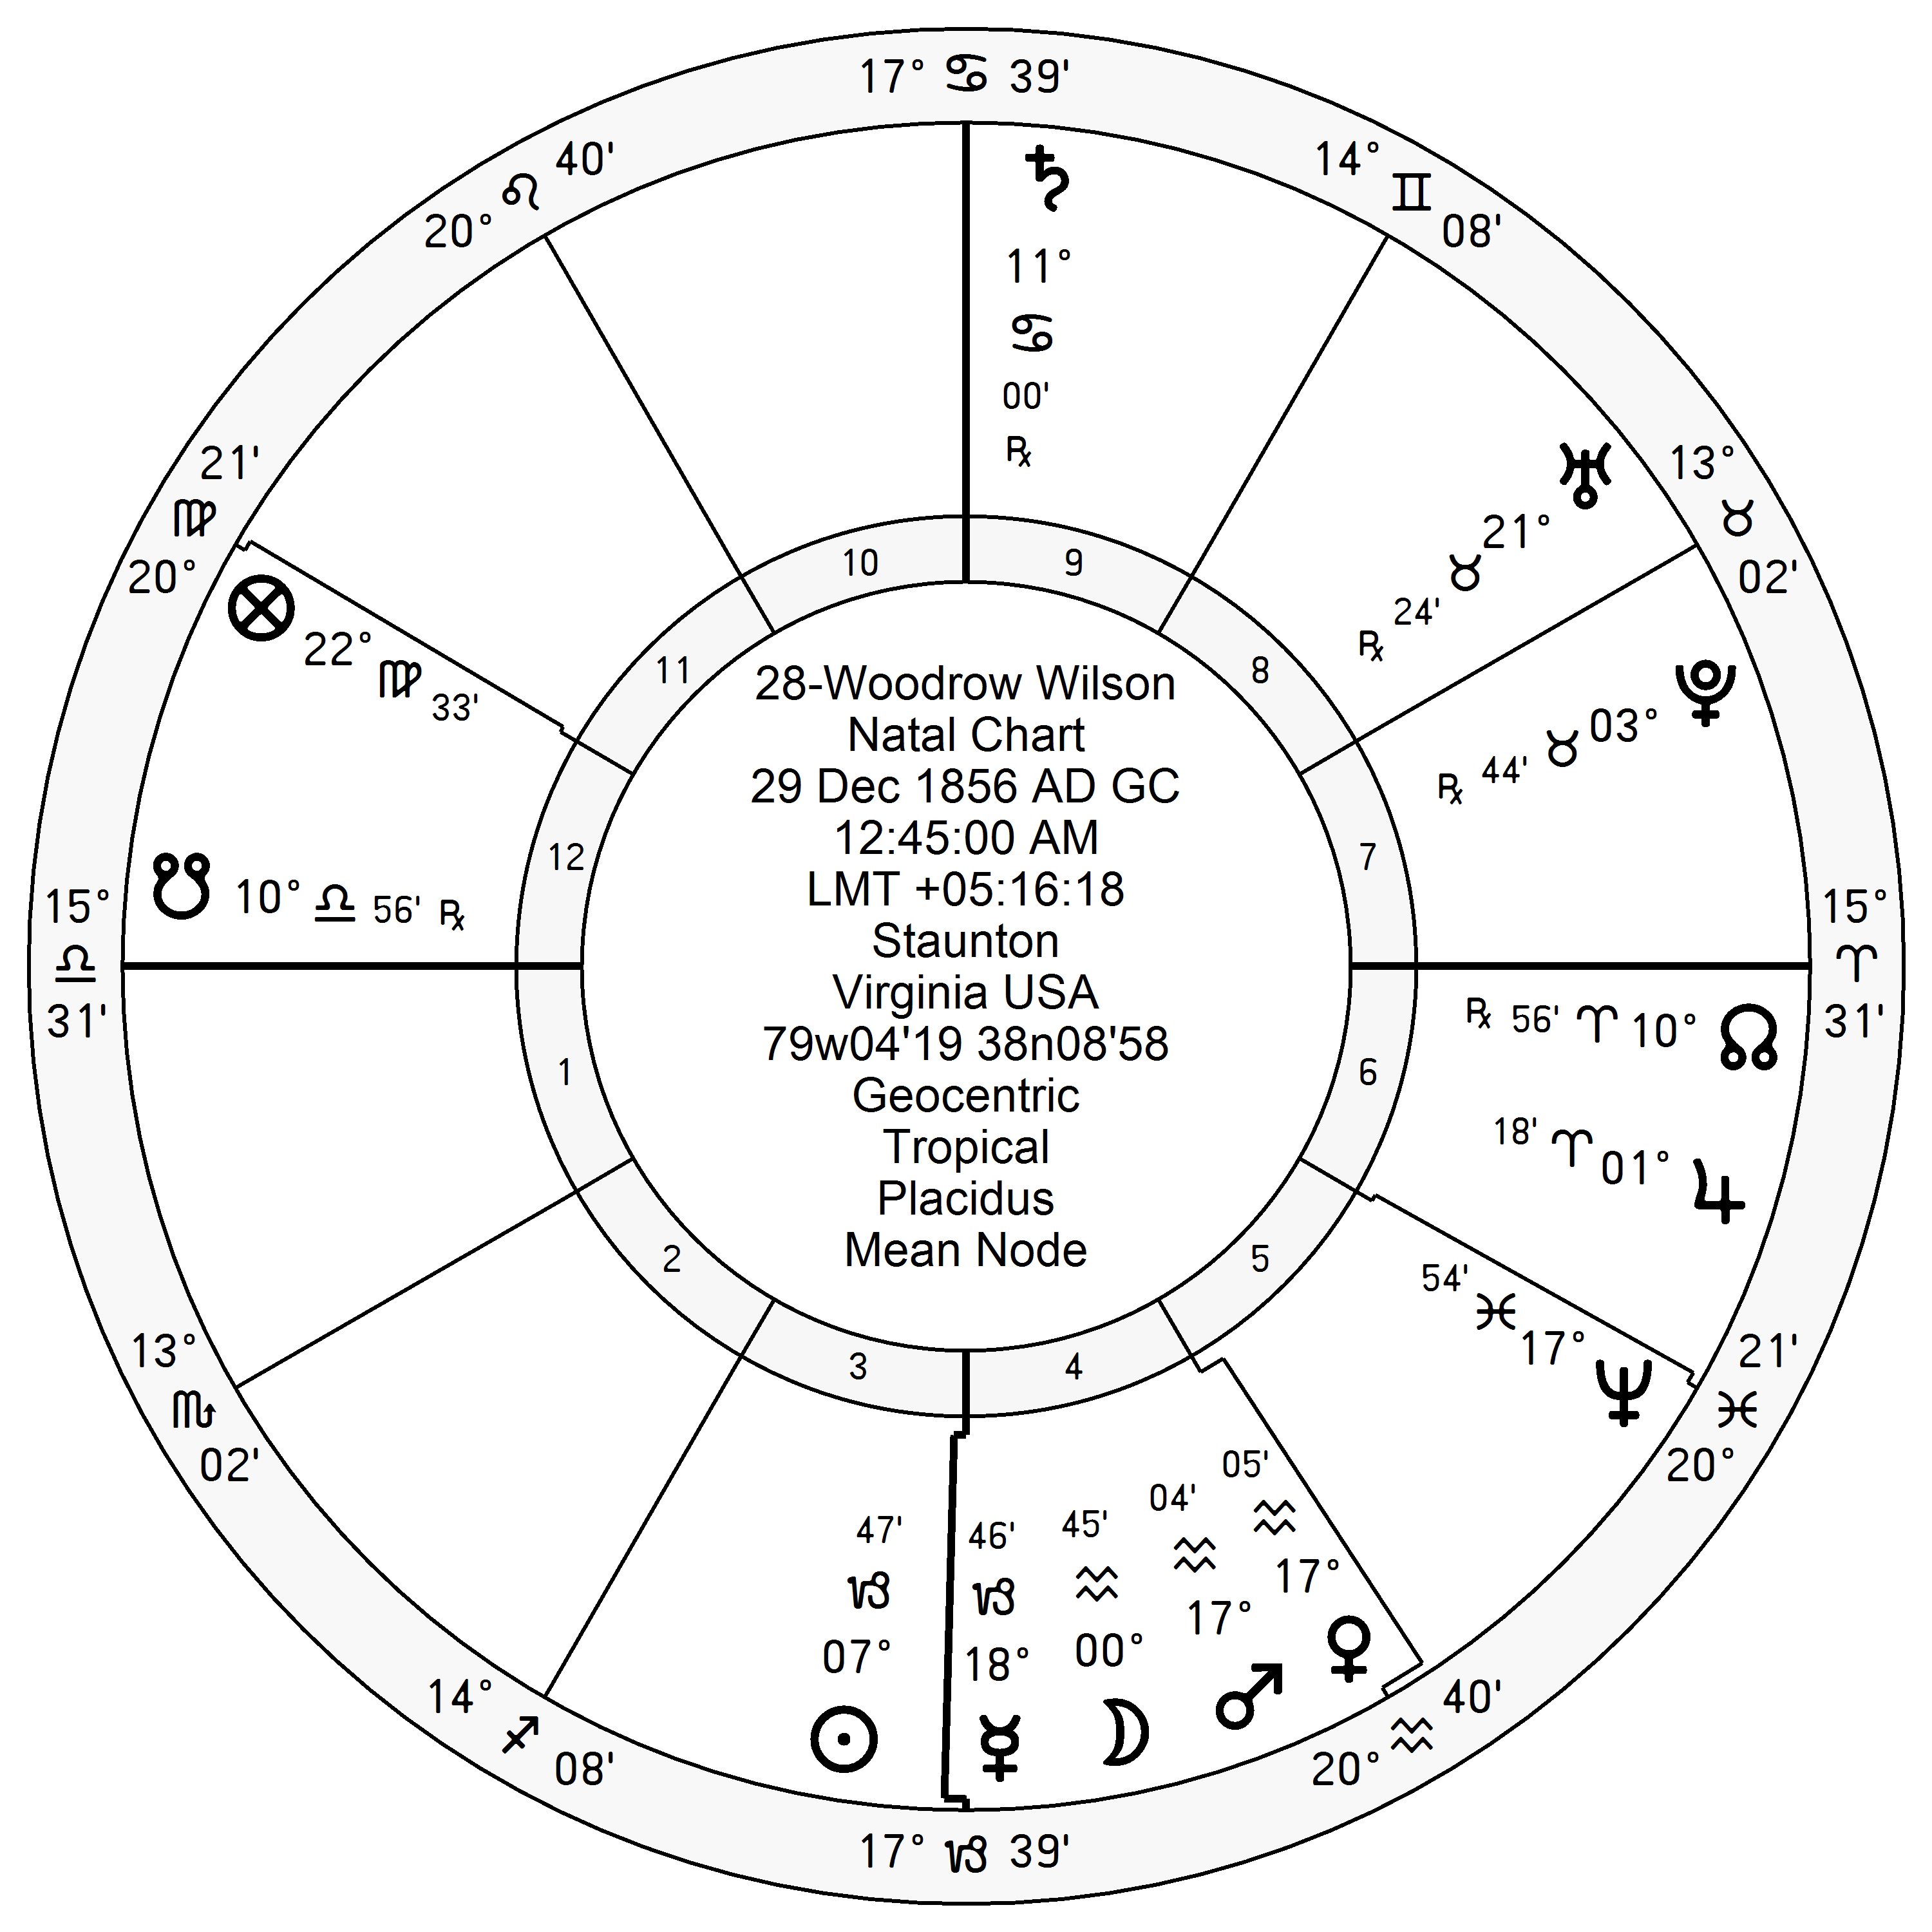
\includegraphics[width=0.9\textwidth]{charts/Wilson.png}}
\fontsize{7pt}{8pt}\selectfont

\Mercury\, \Opposition\, N10; \Trine\, P1, \Square\, N1 \\
\Moon\, \Trine\, N1


\column{0.48\textwidth}
\vspace{-1em}
{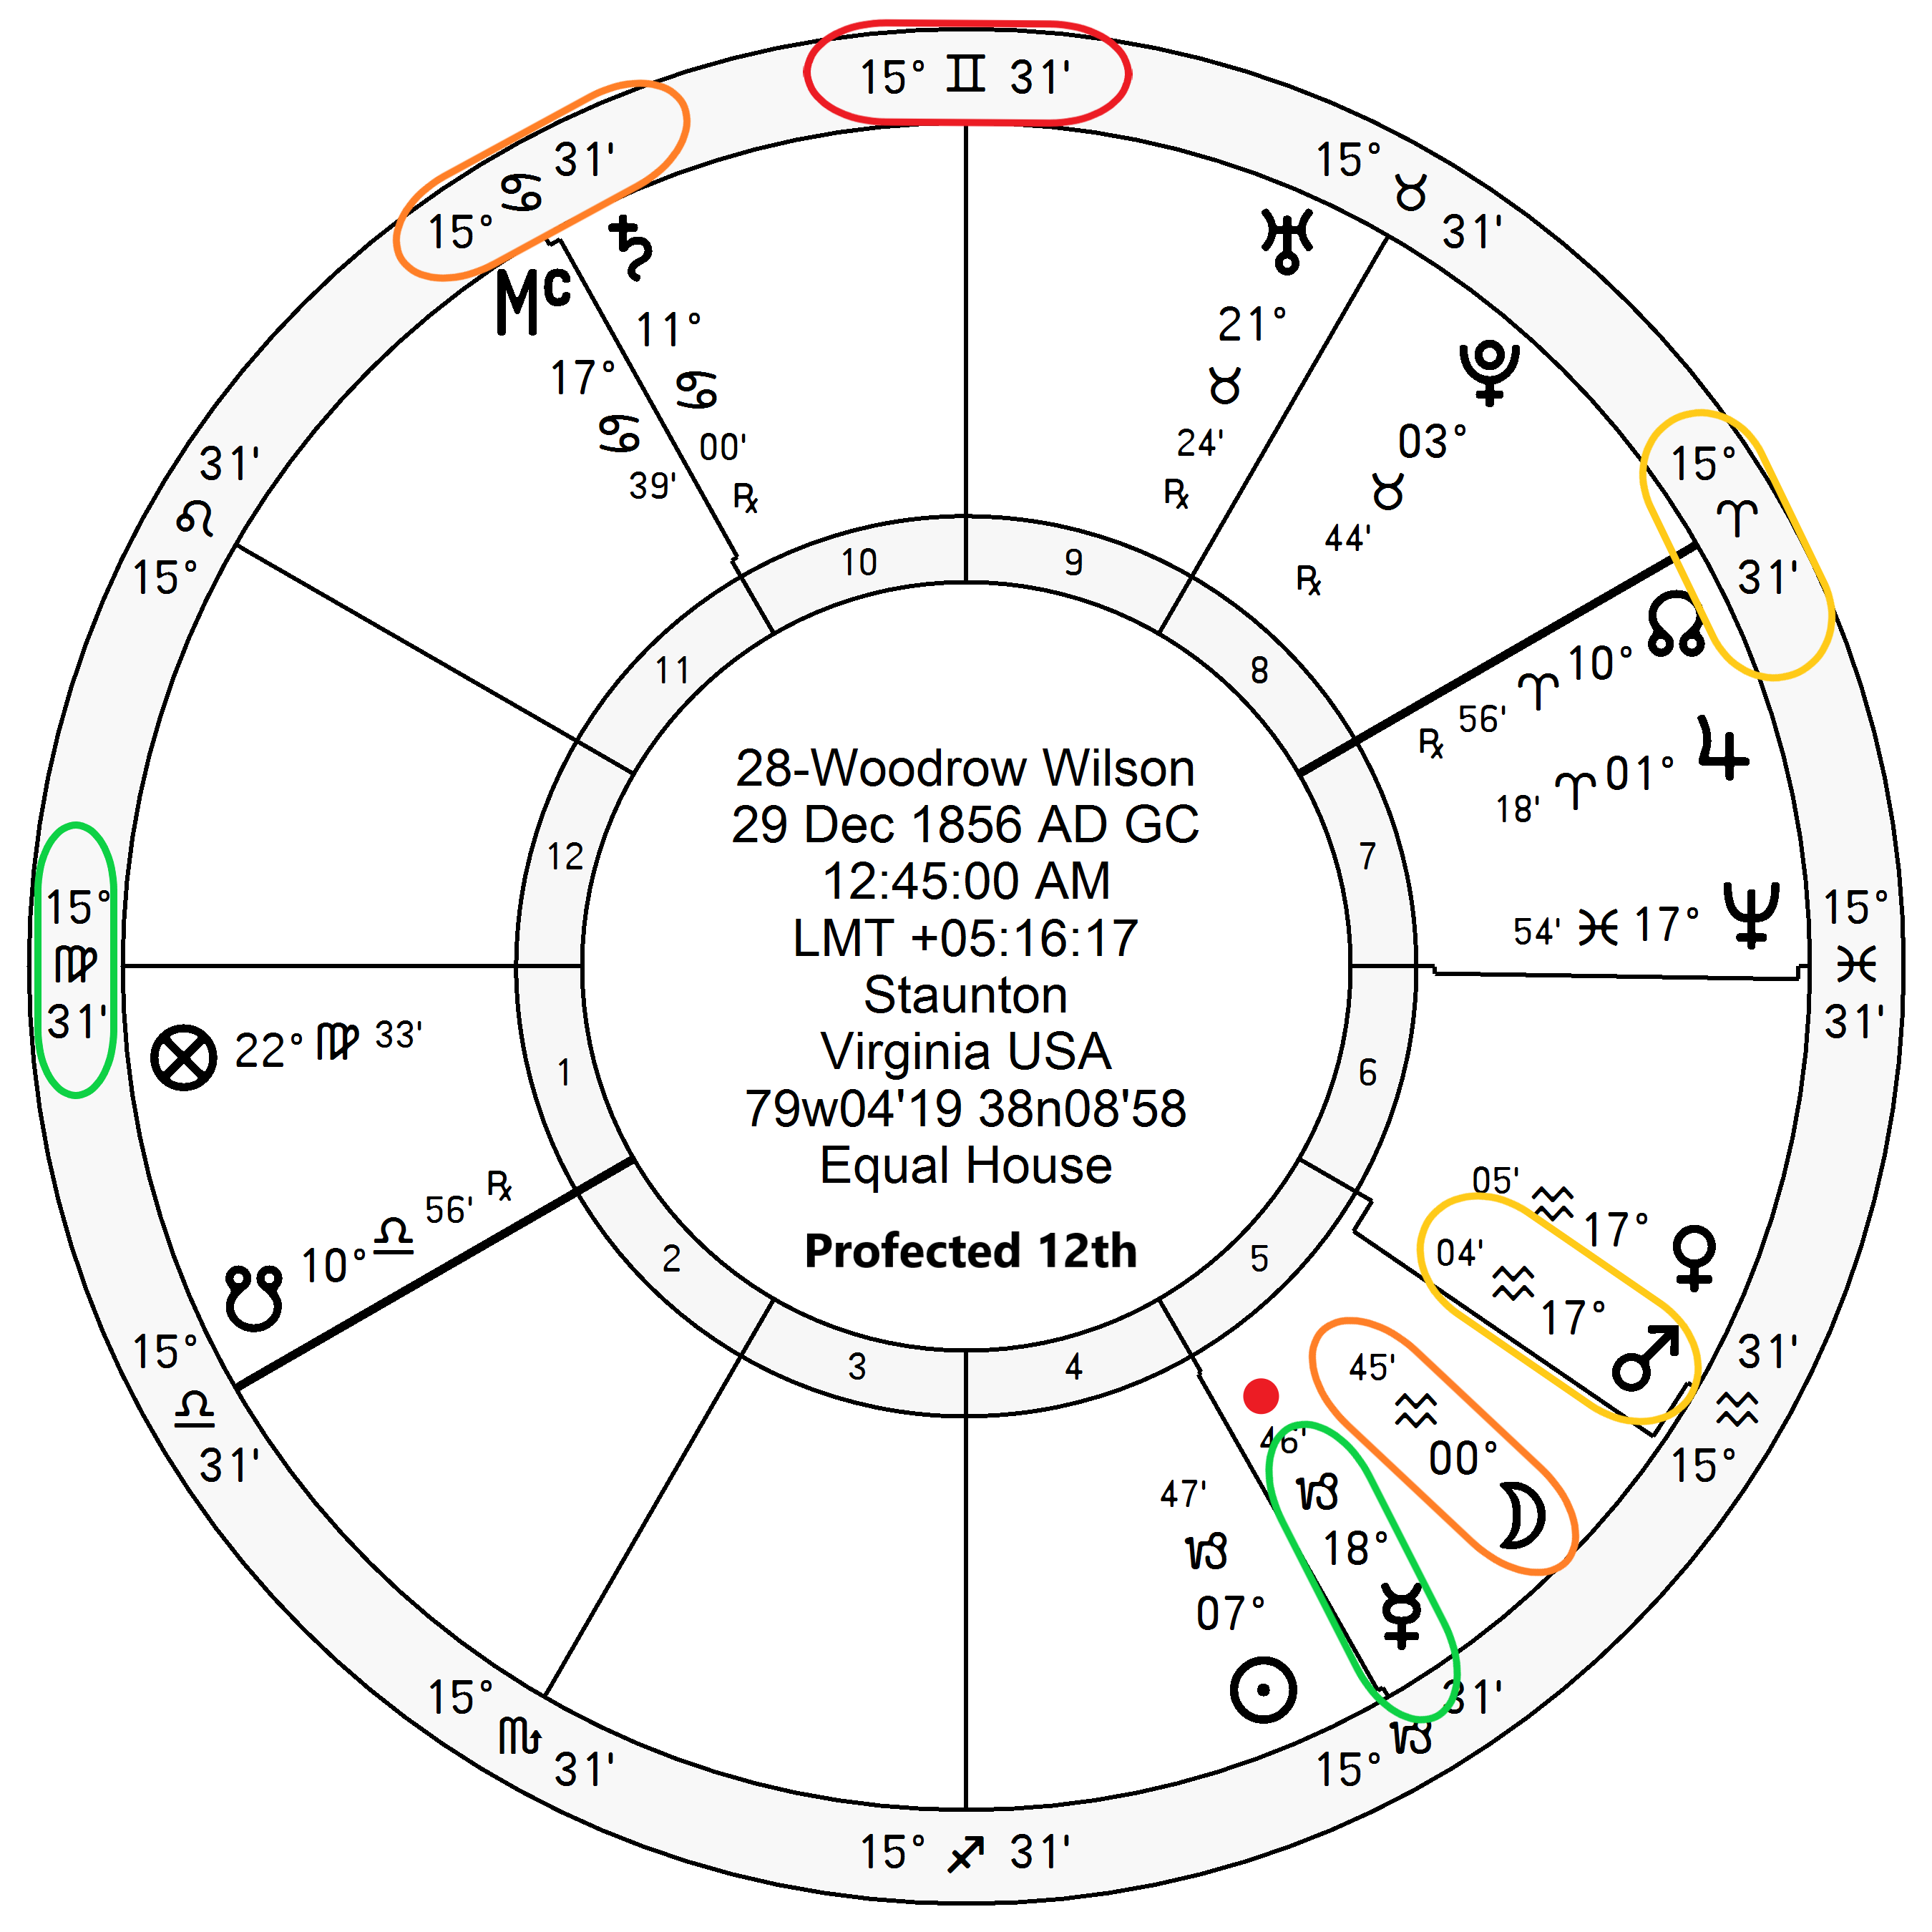
\includegraphics[width=0.9\textwidth]{charts/Wilson-Prof-12th.png}}
\textbf{\dgreen P1}=N12
	$\Rightarrow$ \Mercury\, $\Rightarrow$ \textbf{\dgreen P5/N4} \\
\textbf{\red P10}=N9
	$\Rightarrow$  \Mercury\, $\Rightarrow$ \textbf{\dgreen P5/N4} \\
PE=P11/\textbf{\red N10}
	$\Rightarrow$  \Moon\, $\Rightarrow$   \textbf{\dgreen P5/N4}

\end{columns}
\end{frame}

% Roosevelt
\begin{frame}[t]{Election November 7, 1916: Charles Evans Hughes}
\small
\begin{columns}[T, onlytextwidth]
\column{0.48\textwidth}
\vspace{-1em}
{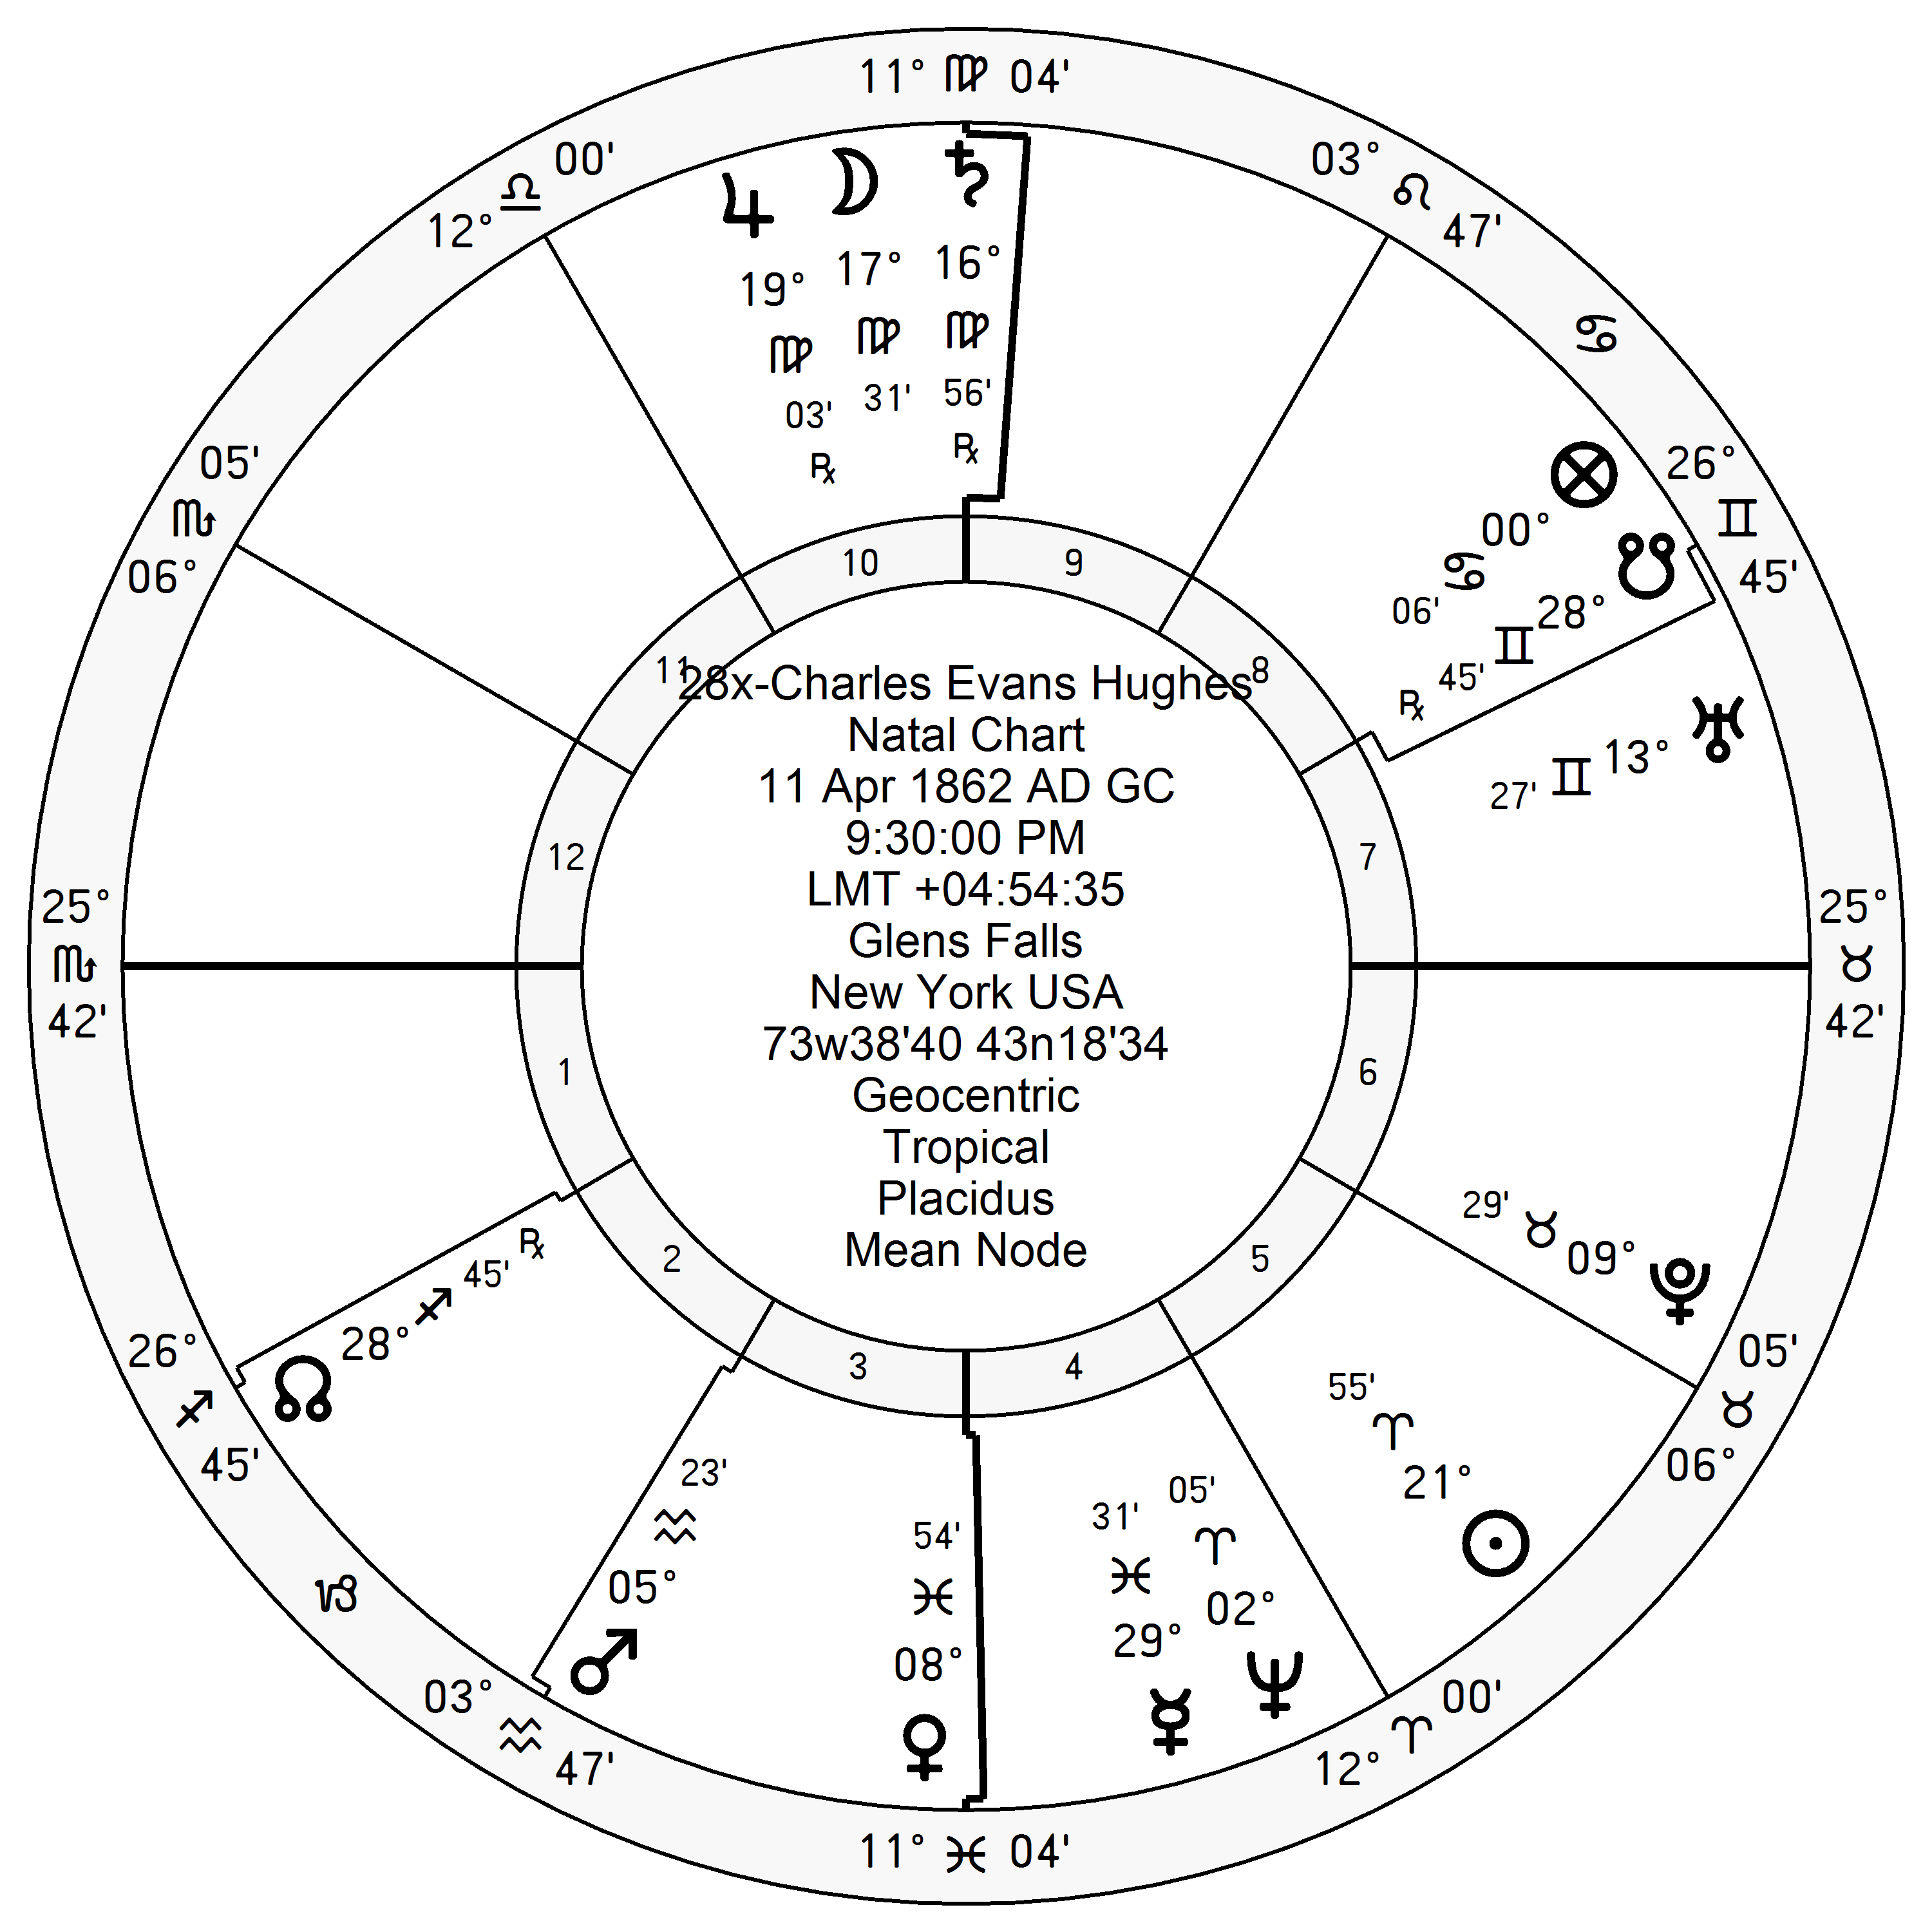
\includegraphics[width=0.9\textwidth]{charts/Hughes.png}}
\fontsize{8pt}{9pt}\selectfont

\Venus\, in P10, \Square\, P1, N1 \\
\Saturn\, \Opposition\, \Venus\, in P10, \Square\, P1; in N10 \\
\Mars\, \Trine\, P1, \Sextile\, N1 \\
\vspace{1em}
\Saturn\, in bad state (retro, disposited by \Mercury\, in Fall; \Square\, \Uranus) denies what the 10th promises?

\column{0.48\textwidth}
\vspace{-1em}
{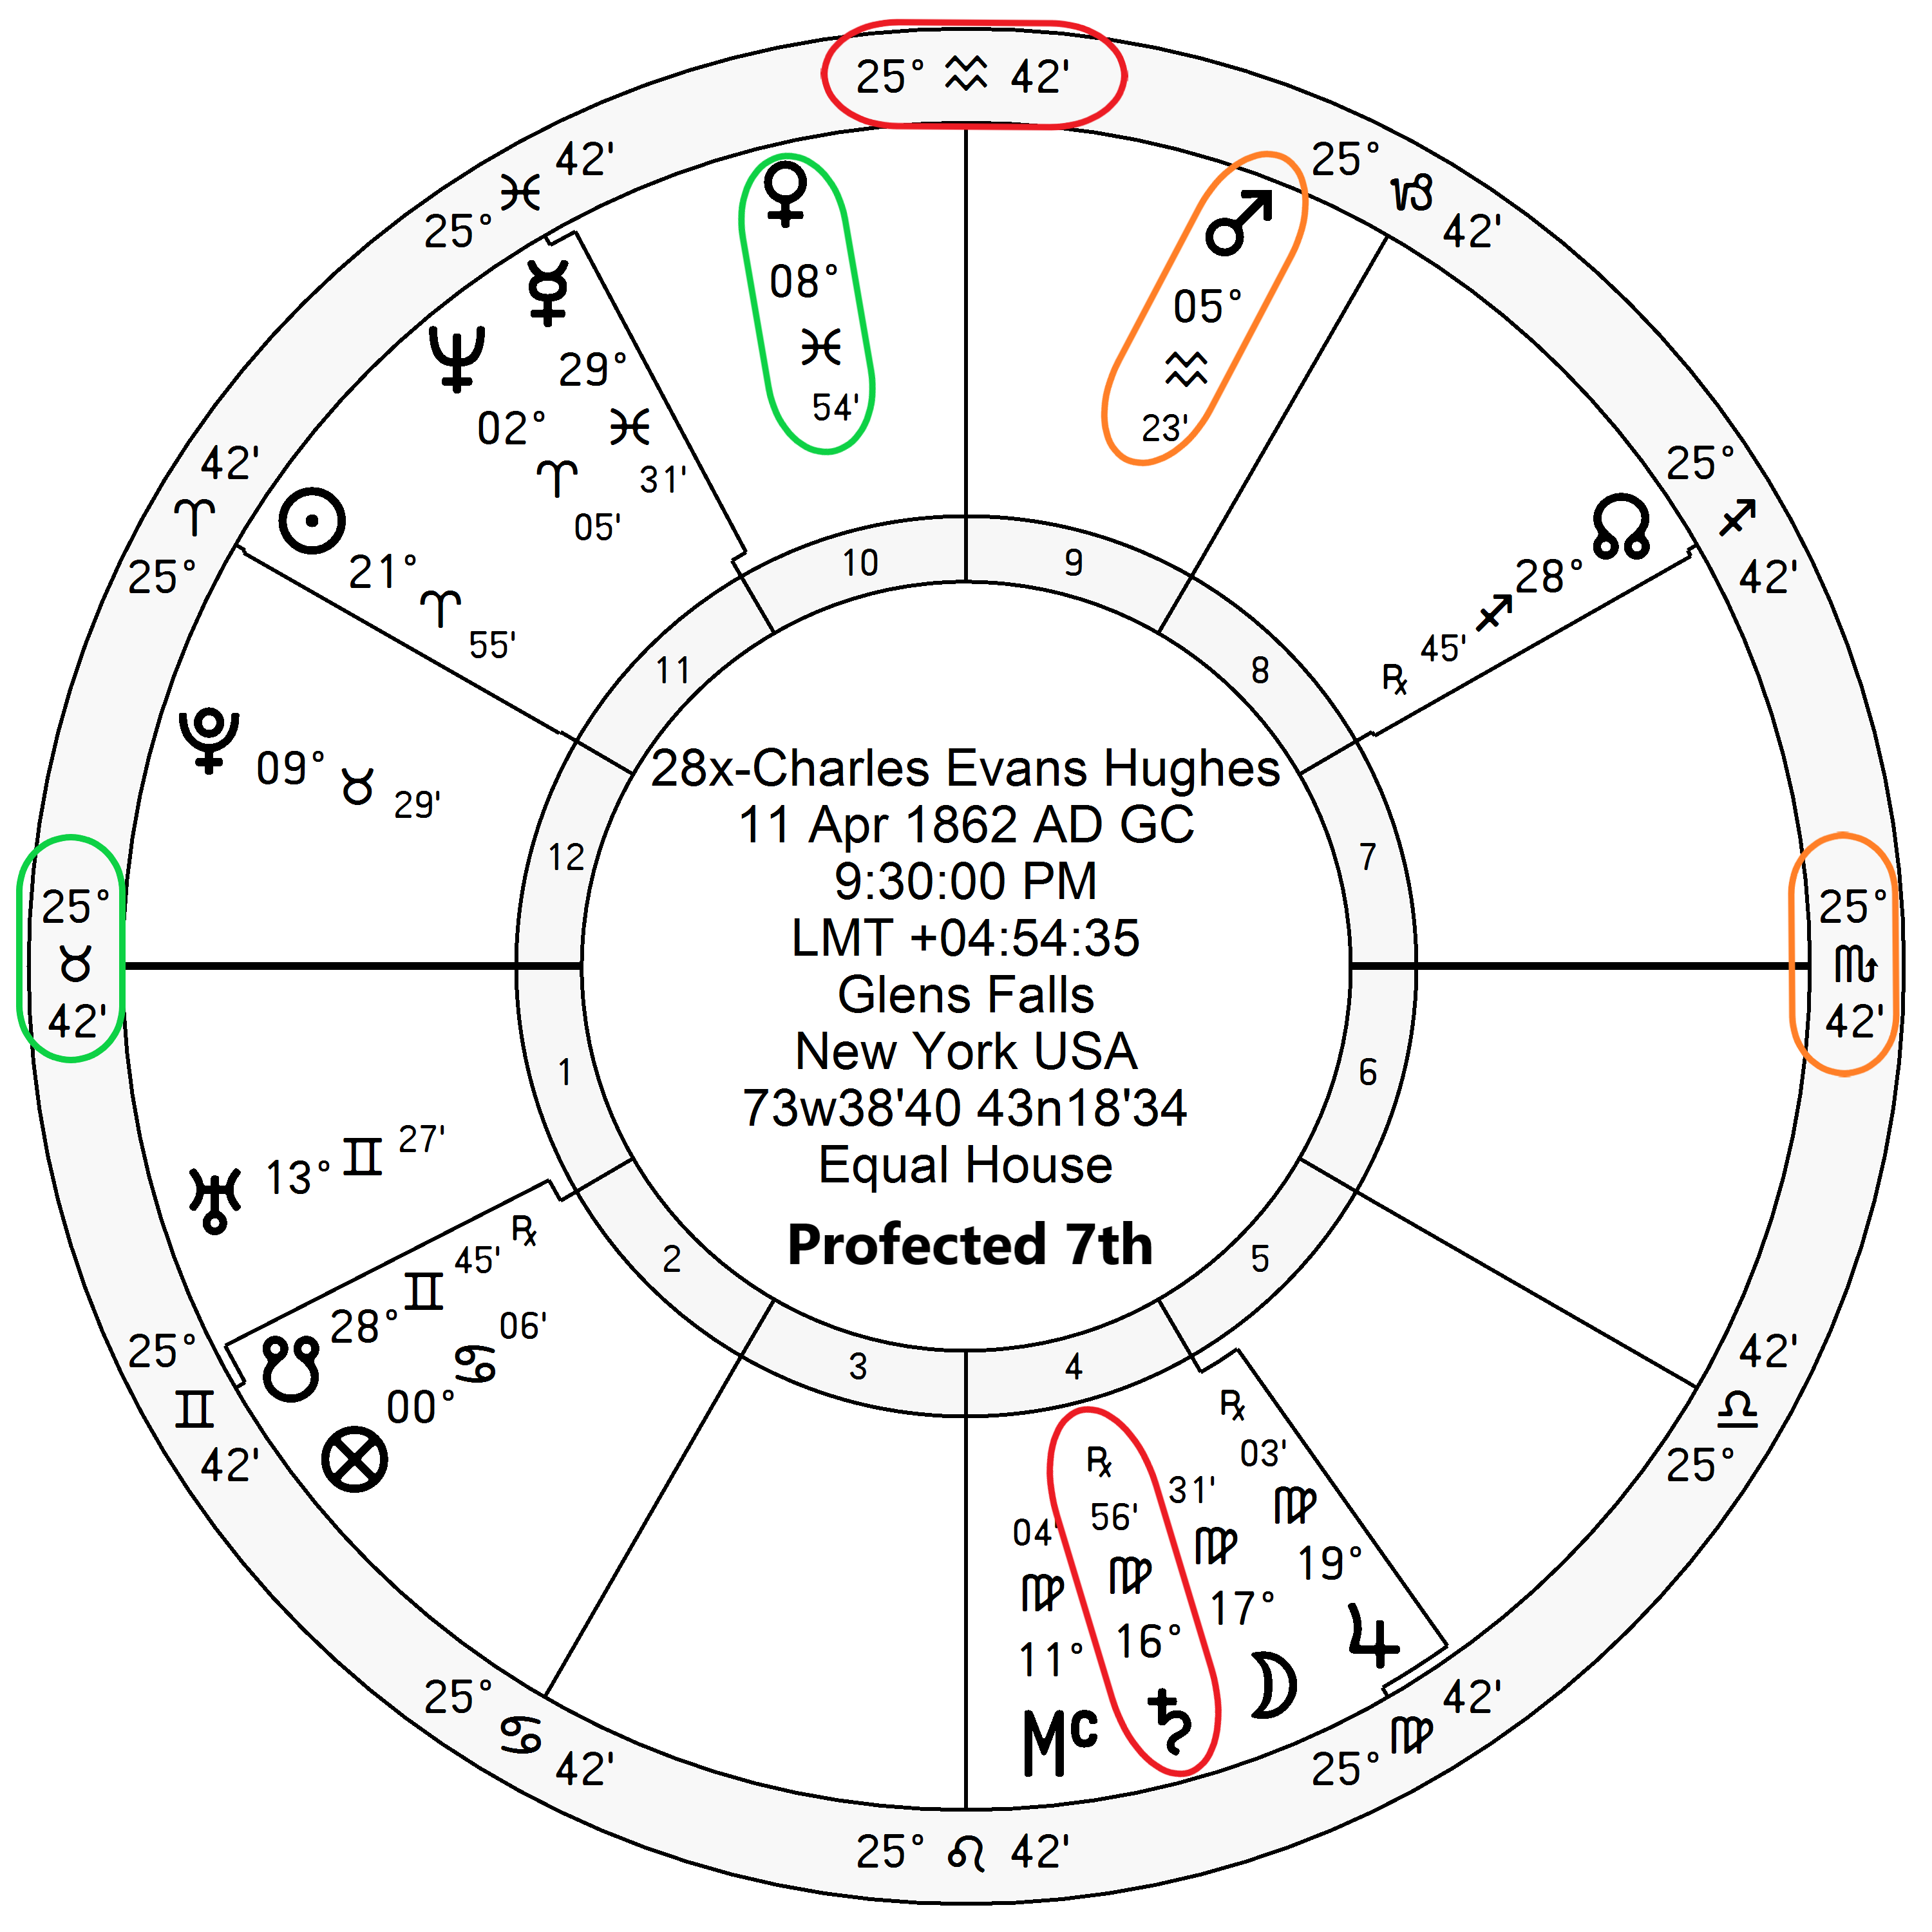
\includegraphics[width=0.9\textwidth]{charts/Hughes-Prof-7th.png}}
\textbf{\dgreen P1=N7} 
	$\Rightarrow$ \Venus\, $\Rightarrow$ \textbf{\red P10/N3}\\
\textbf{\red P10=N3}
	$\Rightarrow$ \Saturn\,\Retrograde $\Rightarrow$ P4/\textbf{\red N10}\\
PE=\textbf{\dgreen P7/}N12
	$\Rightarrow$ \Mars\, $\Rightarrow$ P9/\textbf{\red N3}


\end{columns}
\end{frame}
